\documentclass[aspectratio=169]{beamer}

\usepackage[utf8]{inputenc}

\usepackage{standalone}
\usepackage{caption}
\usepackage{amssymb, amsmath, amsthm, amsfonts}

\usepackage{tikz}
\usepackage{pgfplots}
\usetikzlibrary{shapes.geometric, arrows}
\usetikzlibrary{backgrounds}
\tikzstyle{node} = [rectangle]

\usepackage{float}

\newcommand{\comment}[1]{}

\usetheme{Dresden}
\usepackage[orientation=landscape,size=custom,width=16,height=9,scale=0.5,debug]{beamerposter}
\usepackage{animate}
\usepackage{url}

\title{N-body memory layout exploration}
\author{Oliver Geisel \& Lisa Hentschke}
\date{\today}


\begin{document}

\begin{frame}
	\titlepage
\end{frame}

\begin{frame}
	\frametitle{Structure}
	\tableofcontents
\end{frame}

\section{The task} 
\begin{frame}
	\frametitle{The n-body simulation}
	\begin{columns}
	\begin{column}{0.55\textwidth}
		\begin{itemize}
			\item simulate the interaction of \(n\) particles
			\item each particle has
			\begin{itemize}
				\smallskip
				\item position x
				\item position y
				\item position z
				\smallskip
				\item velocity x
				\item velocity y
				\item velocity z
				\smallskip
				\item mass
			\end{itemize}
		\end{itemize}
	\end{column}
	
	\begin{column}{0.45\textwidth}
		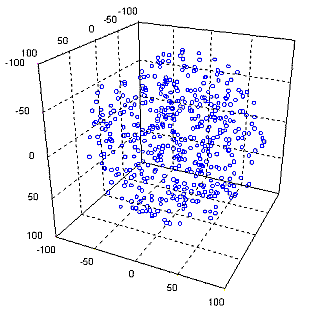
\includegraphics[scale=0.65]{resources/nbody.png}
		\tiny \url{http://astro.dur.ac.uk/~nm/pubhtml/nbody/nbody.html}
	\end{column}
	
	\end{columns}
	
\end{frame}

\section{Solution Strategies}
\begin{frame}
	\frametitle{Solution Strategies}
	\begin{itemize}
		\item rewrite CPP-code in CUDA: implement AoS, SoA and AoSoA memory layouts
		\item implemented \underline{shared memory} variants
		\item for SoA: implemented two sub-variants: B and T
			\begin{itemize}
				\item B: compute one particle per block
				\item T: compute one particle per thread
			\end{itemize}
		\item We tested on K80 (Taurus), v100 (Taurus), 1070 (private, driver version 461.09), and RTX 2080 (private) respectively
	\end{itemize}
\end{frame}

\begin{frame}
	\frametitle{Example on K80}
	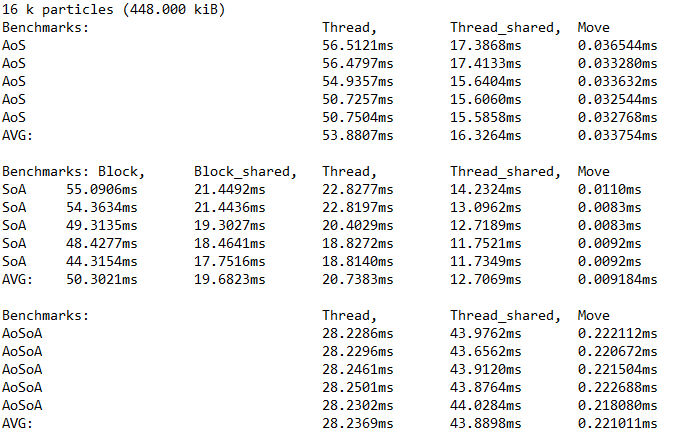
\includegraphics[scale=0.5]{resources/data-example.png}
\end{frame}


\section{Results}
\begin{frame}
	\frametitle{Used Profilers}
	\begin{columns}
	\begin{column}{0.3\textwidth}
		\begin{itemize}
			\small \item nvprof on Taurus
		\end{itemize}
	\end{column}
	
	\begin{column}{0.5\textwidth}
		\begin{itemize}
			\small \item Nvidia Visual Profiler version 11.2
		\end{itemize}
	\end{column}
	\end{columns}
	\medskip
	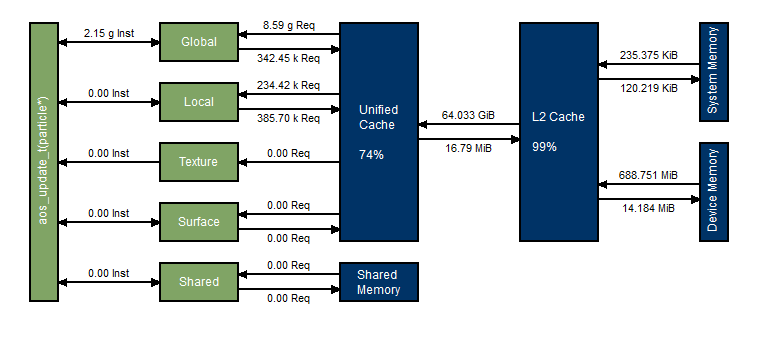
\includegraphics[scale=0.50]{resources/128-1070-aos-update-t.png}
	\smallskip
	\small tested on 1070; version 128k paricles on mem layout AoS; subversion T
\end{frame}

\begin{frame}
	\frametitle{Used Profilers}
	\begin{columns}
	\begin{column}{0.3\textwidth}
		\begin{itemize}
			\small \item nvprof on Taurus
		\end{itemize}
	\end{column}
	
	\begin{column}{0.5\textwidth}
		\begin{itemize}
			\small \item Nvidia Visual Profiler version 11.2
		\end{itemize}
	\end{column}
	\end{columns}
	\smallskip
	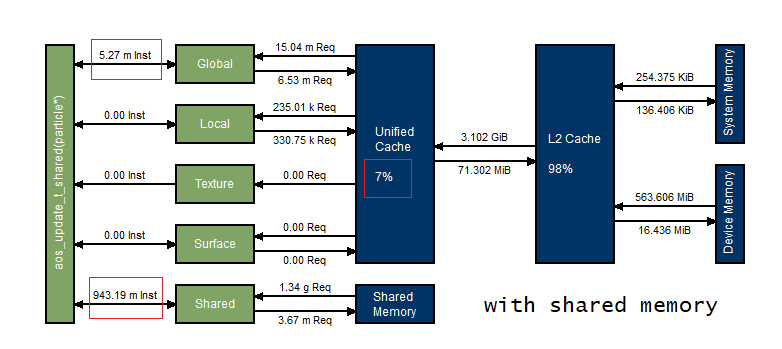
\includegraphics[scale=0.50]{resources/128-1070-aos-update-t-shared.png}
	\smallskip
	\small tested on 1070; version 128k paricles on mem layout AoS; subversion T
\end{frame}


\begin{frame}
	\frametitle{Compare the memory structures - on K80}
	\begin{columns}
	\begin{column}{0.25\textwidth}
	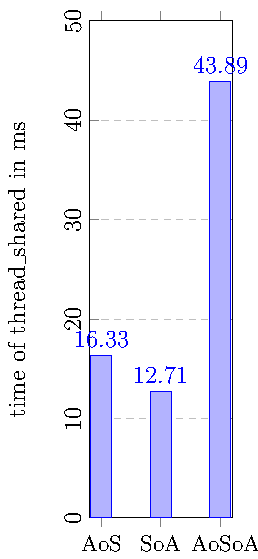
\includegraphics[scale=0.55]{figures/fig1.pdf}
	\small 16K
	\end{column}
	%===========
	\begin{column}{0.25\textwidth}
	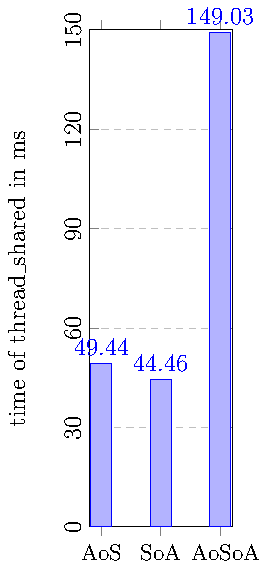
\includegraphics[scale=0.55]{figures/fig2.pdf}
	\small 32K
	\end{column}
	%===========
	\begin{column}{0.25\textwidth}
	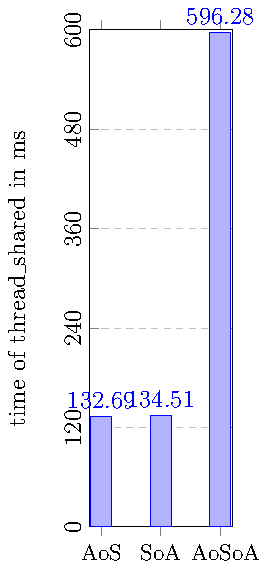
\includegraphics[scale=0.55]{figures/fig3.pdf}
	\small 64K
	\end{column}
	%===========
	\begin{column}{0.25\textwidth}
	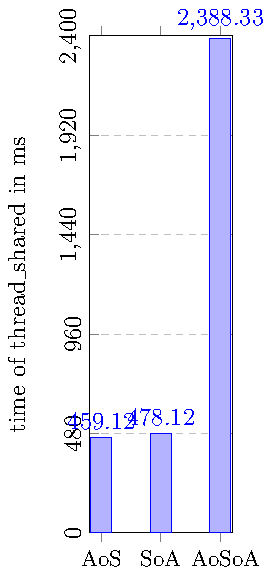
\includegraphics[scale=0.55]{figures/fig4.pdf}
	\small 128K
	\end{column}	
	\end{columns}
	
\end{frame}


\begin{frame}
	\frametitle{Compare the memory structures - on v100}
	\begin{columns}
	\begin{column}{0.25\textwidth}
	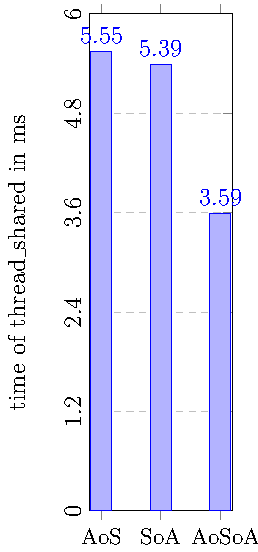
\includegraphics[scale=0.55]{figures/fig10.pdf}
	\small 16K
	\end{column}
	%===========
	\begin{column}{0.25\textwidth}
	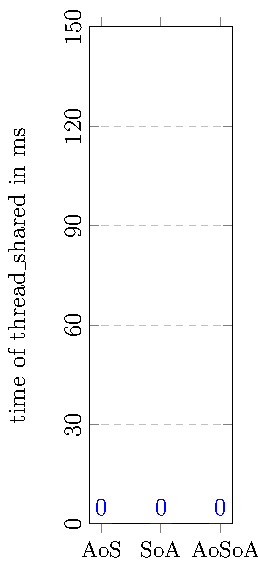
\includegraphics[scale=0.55]{figures/fig20.pdf}
	\small 32K
	\end{column}
	%===========
	\begin{column}{0.25\textwidth}
	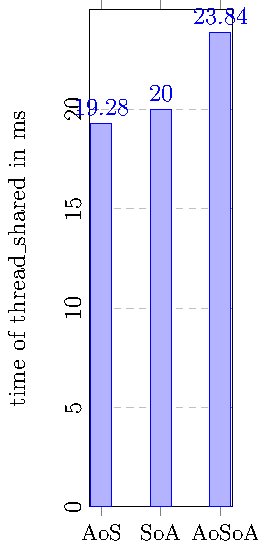
\includegraphics[scale=0.55]{figures/fig30.pdf}
	\small 64K
	\end{column}
	%===========
	\begin{column}{0.25\textwidth}
	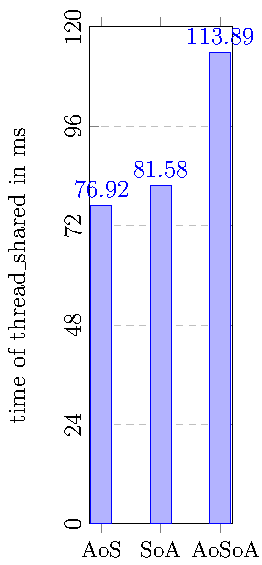
\includegraphics[scale=0.55]{figures/fig40.pdf}
	\small 128K
	\end{column}	
	\end{columns}
	
\end{frame}


\begin{frame}
	\frametitle{Compare the memory structures - on 1070}
	\begin{columns}
	\begin{column}{0.25\textwidth}
	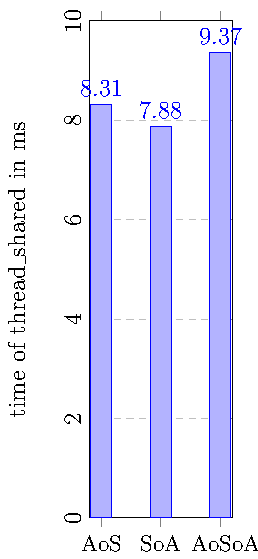
\includegraphics[scale=0.55]{figures/fig100.pdf}
	\small 16K
	\end{column}
	%===========
	\begin{column}{0.25\textwidth}
	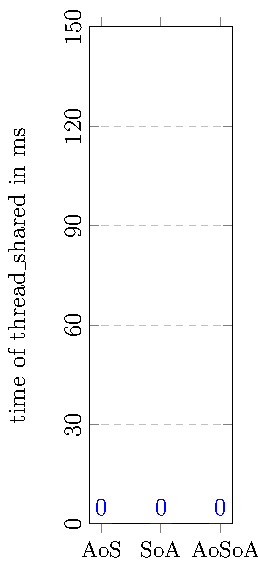
\includegraphics[scale=0.55]{figures/fig200.pdf}
	\small 32K
	\end{column}
	%===========
	\begin{column}{0.25\textwidth}
	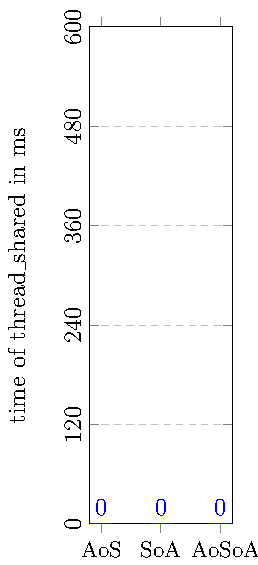
\includegraphics[scale=0.55]{figures/fig300.pdf}
	\small 64K
	\end{column}
	%===========
	\begin{column}{0.25\textwidth}
	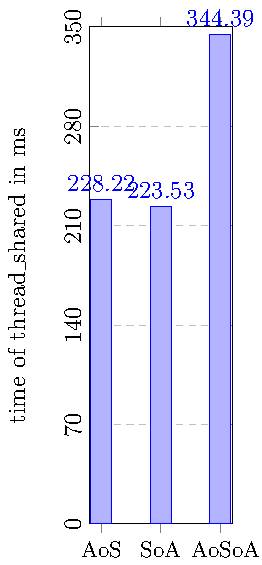
\includegraphics[scale=0.55]{figures/fig400.pdf}
	\small 128K
	\end{column}	
	\end{columns}
	
\end{frame}


\begin{frame}
	\frametitle{Compare the memory structures - on RTX 2080}
	\begin{columns}
	\begin{column}{0.25\textwidth}
	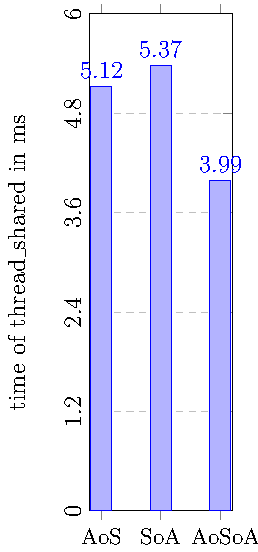
\includegraphics[scale=0.55]{figures/fig1000.pdf}
	\small 16K
	\end{column}
	%===========
	\begin{column}{0.25\textwidth}
	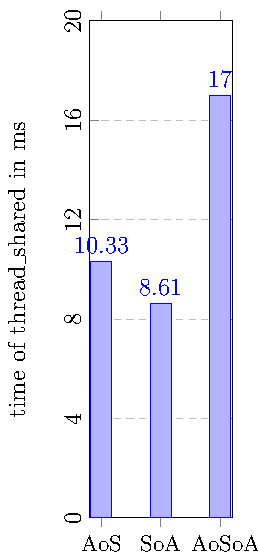
\includegraphics[scale=0.55]{figures/fig2000.pdf}
	\small 32K
	\end{column}
	%===========
	\begin{column}{0.25\textwidth}
	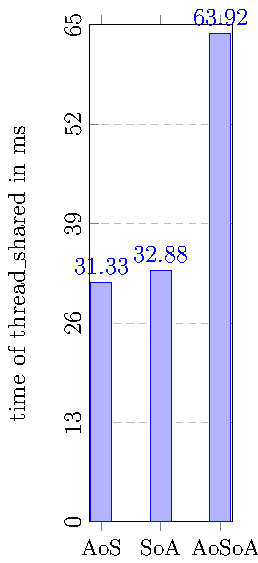
\includegraphics[scale=0.55]{figures/fig3000.pdf}
	\small 64K
	\end{column}
	%===========
	\begin{column}{0.25\textwidth}
	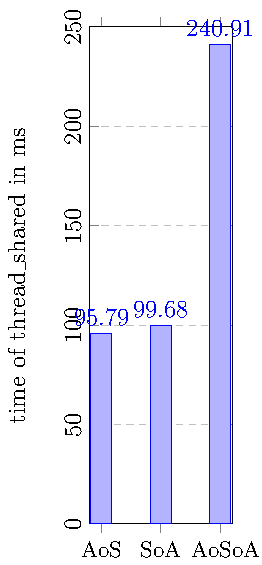
\includegraphics[scale=0.55]{figures/fig4000.pdf}
	\small 128K
	\end{column}	
	\end{columns}
	
\end{frame}

\section{Explanation}
\begin{frame}
	\frametitle{Why?}
	Memory Layout:
	\begin{itemize}
		\item K80 - GDDR 5 with SDRAM
		\item v100 - HBM 2
		\item 1070 - GDDR 5
		\item RTX 2080 - GDDR 6
	\end{itemize}
\end{frame}

\section{Further Approaches}
\begin{frame}
	\frametitle{What else could we try?}
	\begin{itemize}
		\item use texture memory
		\item change computation (not part of the task)
	\end{itemize}
\end{frame}

\end{document}